% -*- latex -*-
%%%%%%%%%%%%%%%%%%%%%%%%%%%%%%%%%%%%%%%%%%%%%%%%%%%%%%%%%%%%%%%%
%%%%%%%%%%%%%%%%%%%%%%%%%%%%%%%%%%%%%%%%%%%%%%%%%%%%%%%%%%%%%%%%
%%%%
%%%% This text file is part of the lecture slides for
%%%% `Parallel Computing'
%%%% by Victor Eijkhout, copyright 2012-9
%%%%
%%%% Graph-slides.tex : slides about MPI graph topologies
%%%%
%%%%%%%%%%%%%%%%%%%%%%%%%%%%%%%%%%%%%%%%%%%%%%%%%%%%%%%%%%%%%%%%
%%%%%%%%%%%%%%%%%%%%%%%%%%%%%%%%%%%%%%%%%%%%%%%%%%%%%%%%%%%%%%%%

\begin{frame}[containsverbatim]{Overview}
  This section discusses graph topologies.

  Commands learned:
  \begin{itemize}
  \item \indexmpishow{MPI_Dist_graph_create}, \indexmpishow{MPI_DIST_GRAPH}
  \item \indexmpishow{MPI_Neighbor_...}
  \end{itemize}
\end{frame}

\begin{frame}[containsverbatim]{Process topologies}
  \begin{itemize}
  \item Processes don't communicate at random
  \item Example: Cartesian grid, each process 4 (or so) neighbours
  \item Express operations in terms of topology
  \item Elegance of expression
  \end{itemize}
\end{frame}

\begin{frame}[containsverbatim]{Process reordering}
  \begin{itemize}
  \item Consecutive process numbering often the best:\\
    divide array by chunks
  \item Not optimal for grids or general graphs:
  \item MPI is allowed to renumbering ranks
  \item Graph topology gives information from which to deduce
    renumbering
  \end{itemize}
\end{frame}

\begin{frame}[containsverbatim]{MPI-1 topology}
  \begin{itemize}
  \item Cartesian topology
  \item Graph topology, globally specified.\\
    Not exactly scalable!
  \end{itemize}
\end{frame}

\begin{frame}[containsverbatim]{MPI-2  and 3 topology}
  \begin{itemize}
  \item Graph topologies locally specified: scalable!
  \item Neighborhood collectives:\\
    expression close to the algorith.
  \end{itemize}
\end{frame}

\begin{frame}{Neighbourhood collective}
  \label{fig:graphcollective}
  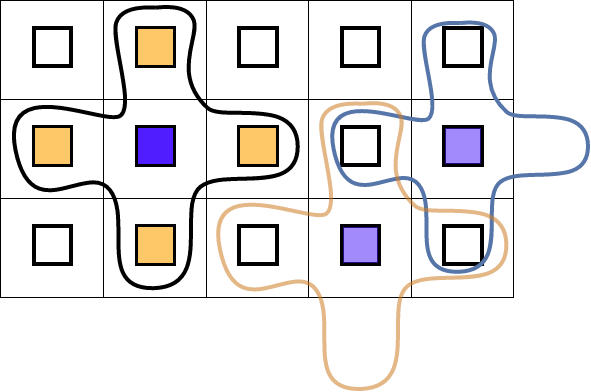
\includegraphics[scale=.5]{graphcollective}

  Distributed graph topology where each
  node has four neighbours
\end{frame}

\begin{frame}[containsverbatim]{Whyy neighbourhood collectives?}
  \begin{itemize}
  \item Using \indexmpishow{MPI_Isend}~/ \indexmpishow{MPI_Irecv} is like spelling out a collective;
  \item Collectives can use pipelining as opposed to sending a whole
    buffer;
  \item Collectives can use spanning trees as opposed to direct connections.
  \end{itemize}
\end{frame}

\begin{frame}[containsverbatim]{Create graph topology}
\lstset{language=C}
\begin{lstlisting}
int MPI_Dist_graph_create
   (MPI_Comm comm_old, int n, const int sources[],
    const int degrees[], const int destinations[], const int weights[],
    MPI_Info info, int reorder,
    MPI_Comm *comm_dist_graph)
\end{lstlisting}
\begin{itemize}
\item \lstinline{nsources} how many processes described? (Usually~1)
\item \lstinline{sources} the processes being described (Usually
  \indexmpishow{MPI_Comm_rank} value)
\item \lstinline{degrees} how many processes to send to
\item \lstinline{destinations} their ranks
\item \lstinline{weights}: usually set to \indexmpishow{MPI_UNWEIGHTED}.
\item \lstinline{info}: \indexmpishow{MPI_INFO_NULL} will do
\item \lstinline{reorder}: 1~if dynamically reorder processes
\end{itemize}
\end{frame}

\begin{frame}[containsverbatim]{Neighbourhood collectives}
\begin{lstlisting}
int MPI_Neighbor_allgather
   (const void *sendbuf, int sendcount,MPI_Datatype sendtype,
    void *recvbuf, int recvcount, MPI_Datatype recvtype,
    MPI_Comm comm)
\end{lstlisting}
Like an ordinary \indexmpishow{MPI_Allgather}, but\\
the receive buffer has a length \lstinline{degree}.
\end{frame}

\begin{exerciseframe}[rightgraph]
  \input ex:rightgraph
\end{exerciseframe}

\begin{frame}{Inspiring picture for the previous exercise}
  \label{fig:rightgraph}

  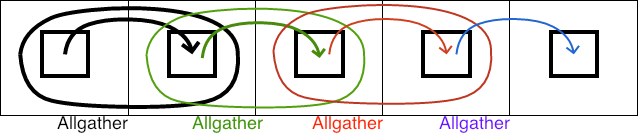
\includegraphics[scale=.5]{rightgraph}

  Solving the right-send exercise with neighbourhood
  collectives
\end{frame}

\endinput

\begin{frame}[containsverbatim]{}
\end{frame}

